\newcommand{\langue}{english}
% Préambule commun aux rapports. Définir \langue (french ou english) avant de l'inclure.
\documentclass[10pt,a4paper,twocolumn]{article}
\usepackage[T1]{fontenc}
\usepackage[utf8]{inputenc}
\usepackage{lmodern}
\usepackage[\langue]{babel}
\usepackage[a4paper,hmargin=1.5cm,top=1.5cm,bottom=2cm]{geometry}
\usepackage{amsmath,amssymb,graphicx,booktabs,enumitem,microtype}
\usepackage[font=small,skip=6pt]{caption}
\usepackage[hidelinks]{hyperref}
\setlength{\columnsep}{0.85cm}
\setlist{leftmargin=1.2em,itemsep=1pt,topsep=3pt,parsep=0pt}
\newcommand{\pa}[1]{\par\smallskip\noindent\textbf{#1}\enspace}
\newcommand{\ket}[1]{\lvert #1\rangle}
\newcommand{\en}[1]{\emph{#1}}
% \entete{titre}{sous-titre}{cadre}{auteurs et lignes suivantes}{nom du résumé}{résumé}
\newcommand{\entete}[6]{%
\twocolumn[\begin{center}
{\LARGE\bfseries #1\par}\vspace{6pt}
{\large #2\par}\vspace{10pt}
{\large\bfseries #3\par}\vspace{2pt}
{#4\par}
\end{center}
\vspace{4pt}
\begin{center}\begin{minipage}{0.9\textwidth}
\begin{center}\bfseries #5\end{center}\vspace{-4pt}
\small #6
\end{minipage}\end{center}
\vspace{14pt}]}
\frenchspacing
\raggedbottom

\hypersetup{pdftitle={SLIC Superpixels: from the Color Image to the Hyperspectral Cube},pdfauthor={Eliott Dionnet, Enguerrand Le Niliot}}
\begin{document}
\entete{SLIC Superpixels: from the Color Image\\ to the Hyperspectral Cube}
{Reimplementation of the algorithm, evaluation on the Berkeley dataset\\ and extension to hyperspectral and volumetric data}
{Project Report -- Image Processing}
{Télécom Paris, 2025, \textsc{Dionnet Eliott} and \textsc{Le Niliot Enguerrand}\\
Paper studied: R. Achanta et al., \emph{SLIC Superpixels Compared to State-of-the-Art Superpixel Methods}, IEEE TPAMI, 2012\\
November 11, 2026}
{Abstract}
{The SLIC algorithm (Simple Linear Iterative Clustering) splits an image into superpixels with a
$k$-means clustering restricted to a local neighborhood, in a space that combines color and position. This
report presents a complete reimplementation in Python, from the initialization on the gradient minimum
to the reattachment of isolated regions, and evaluates it on an image of the Berkeley Segmentation Dataset
against the scikit-image version. With $K = 200$, our implementation reaches a mean undersegmentation error
of 0.094 versus 0.115 for scikit-image, at the cost of a runtime more than twenty times longer. The
method is then extended to hyperspectral images, with a gradient and a distance computed over all
bands (Salinas, 204 bands; Pavia University, 103 bands), and to three-dimensional volumes in the
form of supervoxels. The common thread of the results is the compactness parameter $m$: its useful range depends
entirely on the scale of the signal values. On Salinas in raw radiance, $m$ varies by a factor of 10 with no
measurable effect, whereas on volumes normalized between 0 and 1, going from $m = 10$ to $m = 0.5$ brings the
undersegmentation error of the synthetic sphere from 0.150 down to 0.000.}

\section{Introduction and Context}
A superpixel is a group of neighboring, similar pixels that is then handled as a single unit.
Replacing the hundreds of thousands of pixels of an image
with a few hundred regions that respect its
edges greatly reduces the cost of downstream processing (segmentation, classification, object tracking) without
erasing shape information. A good superpixel method must therefore adhere to the true object boundaries,
produce regions of comparable size and remain fast.

Achanta et al.~\cite{achanta} proposed SLIC, which recasts
the problem as a $k$-means clustering
in a five-dimensional space $[l, a, b, x, y]$, with a
single decisive change: each center only searches for its
pixels in a window of size $2S \times 2S$ around itself. The cost per iteration becomes linear in the number of
pixels $N$ and no longer depends on the number of superpixels $K$.
The paper shows that this very simple method matches or
outperforms the methods of the time, such as the graph-based segmentation
of Felzenszwalb and Huttenlocher~\cite{felzenszwalb}, on the
Berkeley Segmentation Dataset~\cite{martin}.

This project has three goals. The first is to
reimplement SLIC without relying on a superpixel library, in order to understand every step. The second
is to measure the quality of the resulting segmentation with
the metrics of the paper and to study the influence of its
two parameters, $K$ and $m$. The third is to extend the
method beyond the color image: to hyperspectral images, where each pixel carries a spectrum of more than
a hundred bands, and then to three-dimensional volumes.

The report follows this order. Section~\ref{s:algo} describes the algorithm and Section~\ref{s:impl} our implementation. Section~\ref{s:proto}
presents the evaluation protocol, whose results on a
color image are given in Section~\ref{s:color}. Sections~\ref{s:hyper} and~\ref{s:vol}
cover the hyperspectral and volumetric extensions, before
a discussion of the limitations in Section~\ref{s:disc}.

\section{The SLIC Algorithm}\label{s:algo}
\subsection{A Mixed Color and Position Distance}
SLIC works in the CIELAB space, chosen because
Euclidean distances there roughly follow perceived color differences.
A pixel $i$ is described by $[l_i, a_i, b_i, x_i, y_i]$.
The distance between a center $k$ and a pixel $i$ combines a
color distance and a spatial distance:
\begin{align}
d_c &= \sqrt{(l_i - l_k)^2 + (a_i - a_k)^2 + (b_i - b_k)^2},\\
d_s &= \sqrt{(x_i - x_k)^2 + (y_i - y_k)^2},\\
D &= \sqrt{d_c^2 + \left(\frac{d_s}{S}\right)^{2} m^2}.\label{e:D}
\end{align}
The spatial distance is normalized by the grid step $S$,
which sets the expected size of a superpixel, and the compactness parameter
$m$ sets the weight of position against
color. A large $m$ produces nearly square,
regular regions; a small $m$ lets color dominate and
yields regions that follow edges more closely but are
more irregular. The paper recommends $m \in [1, 40]$ for CIELAB colors.

\subsection{The Steps of the Algorithm}
For an image of $N$ pixels and a target number $K$ of
superpixels, the algorithm proceeds as follows.
\begin{enumerate}
\item \textbf{Initial grid.} The centers are placed on a regular grid of step
\begin{equation}
S = \sqrt{N/K},
\end{equation}
so that each superpixel covers $S^2$ pixels on average.
\item \textbf{Move to the gradient minimum.} Each
center is moved to the pixel of lowest gradient
in its $3 \times 3$ neighborhood, to avoid starting on
an edge or on a noisy pixel.
\item \textbf{Local assignment.} Each center compares the distance $D$ of
Equation~\eqref{e:D} to the pixels of the $2S \times 2S$ window around it. A pixel joins the closest center
among those that examined it.
\item \textbf{Update.} Each center becomes the mean
$[l, a, b, x, y]$ of the pixels assigned to it.
\item \textbf{Iteration.} Steps 3 and 4 are repeated until
the centers barely move. The paper
states that ten iterations are enough for most images.
\item \textbf{Connectivity.} Nothing in $k$-means guarantees
that a superpixel is in one piece. Isolated fragments are reattached to a neighboring superpixel.
\end{enumerate}
Since each pixel is only examined by the few
centers whose window covers it, the assignment step
costs $O(N)$ per iteration, whatever the value of $K$. This is the property
that makes SLIC fast.

\section{Our Implementation}\label{s:impl}
Everything is written in Python with NumPy. OpenCV
is only used for the conversion to the Lab space and for the Sobel
filters; no superpixel function is used.
The implementation choices are the following.

\pa{Color and gradient.} The RGB image is converted to
Lab by OpenCV on 8 bits, then the gradient is computed
with $3 \times 3$ Sobel filters on each of the three channels:
\begin{equation}\label{e:G}
G = \sqrt{\sum_{c \in \{L,a,b\}} (\partial_x I_c)^2 + (\partial_y I_c)^2}.
\end{equation}
The paper uses central differences; the Sobel filter
adds a slight smoothing, which stabilizes the choice of centers in noisy areas.

\pa{Iterations and stopping.} Rather than a fixed number of iterations, we stop the loop when the mean spatial
displacement of the centers falls below 0.5 pixel, with a cap of 20 iterations.

\pa{Connectivity.} A depth-first search on the 4-pixel neighborhood
identifies each connected component. A
component of fewer than $S^2/4$ pixels is reattached to the
superpixel with which it shares the longest boundary, and
the labels are renumbered along the way.

\pa{The final number of superpixels.} The step $S$ is rounded
down to an integer, and the grid is laid from
$S/2$ to the edge of the image. The final number of
superpixels $K_f$ therefore differs from $K$ and changes in plateaus:
several values of $K$ give the same step $S$.

\section{Evaluation Protocol}\label{s:proto}
\subsection{Data}
The color part uses image 3096 of the Berkeley Segmentation Dataset~\cite{martin}, of $481 \times 321$ pixels,
which shows a plane against a cloudy sky. Its boundaries
mix a sharp object with soft transitions, which
makes it a good test of boundary adherence. We
use the five human segmentations provided with
the BSDS500 version of the dataset~\cite{arbelaez}, which contain 3
to 11 regions depending on the annotator, and we average the metrics over the five.

\subsection{Metrics}
\pa{Undersegmentation error.} It measures how much
the superpixels leak out of the ground-truth regions.
For reference regions $g_1, \dots, g_M$ and
superpixels $s_j$, the paper defines it as
\begin{equation}\label{e:U}
U = \frac{1}{N}\left[\sum_{i=1}^{M}\Biggl(\sum_{s_j \,:\, |s_j \cap g_i| > B} |s_j|\Biggr) - N\right],
\end{equation}
where $B$ is 5\,\% of the size $|s_j|$ and absorbs small alignment errors.
A superpixel contained in a single
region counts once and a superpixel straddling
two regions counts twice. $U$ is therefore 0 for a
perfect partition and grows with the leakage.

\pa{Boundary recall.} The boundary recall is the fraction of ground-truth boundary pixels that
lie within 2 pixels of a superpixel boundary.
It equals 1 when all the true boundaries are recovered.

\pa{Gradient alignment.} We add an indicator that requires no ground truth, the ratio
between the mean gradient on the superpixel boundaries
and the mean gradient of the whole image:
\begin{equation}
GA = \frac{\operatorname{mean}_{\partial S}\, G}{\operatorname{mean}\, G}.
\end{equation}
A value above 1 means that the boundaries preferentially run
through areas of strong gradient, hence along edges.

\pa{Baseline.} We compare our results to the
\texttt{slic} function of scikit-image~\cite{skimage}, a compiled implementation
of the same method, called with the same $K$ and $m$.

\pa{Execution.} The experiments were run with the
project code on a two-core machine. The timings
are only meaningful relative to one another.

\begin{figure*}[t]
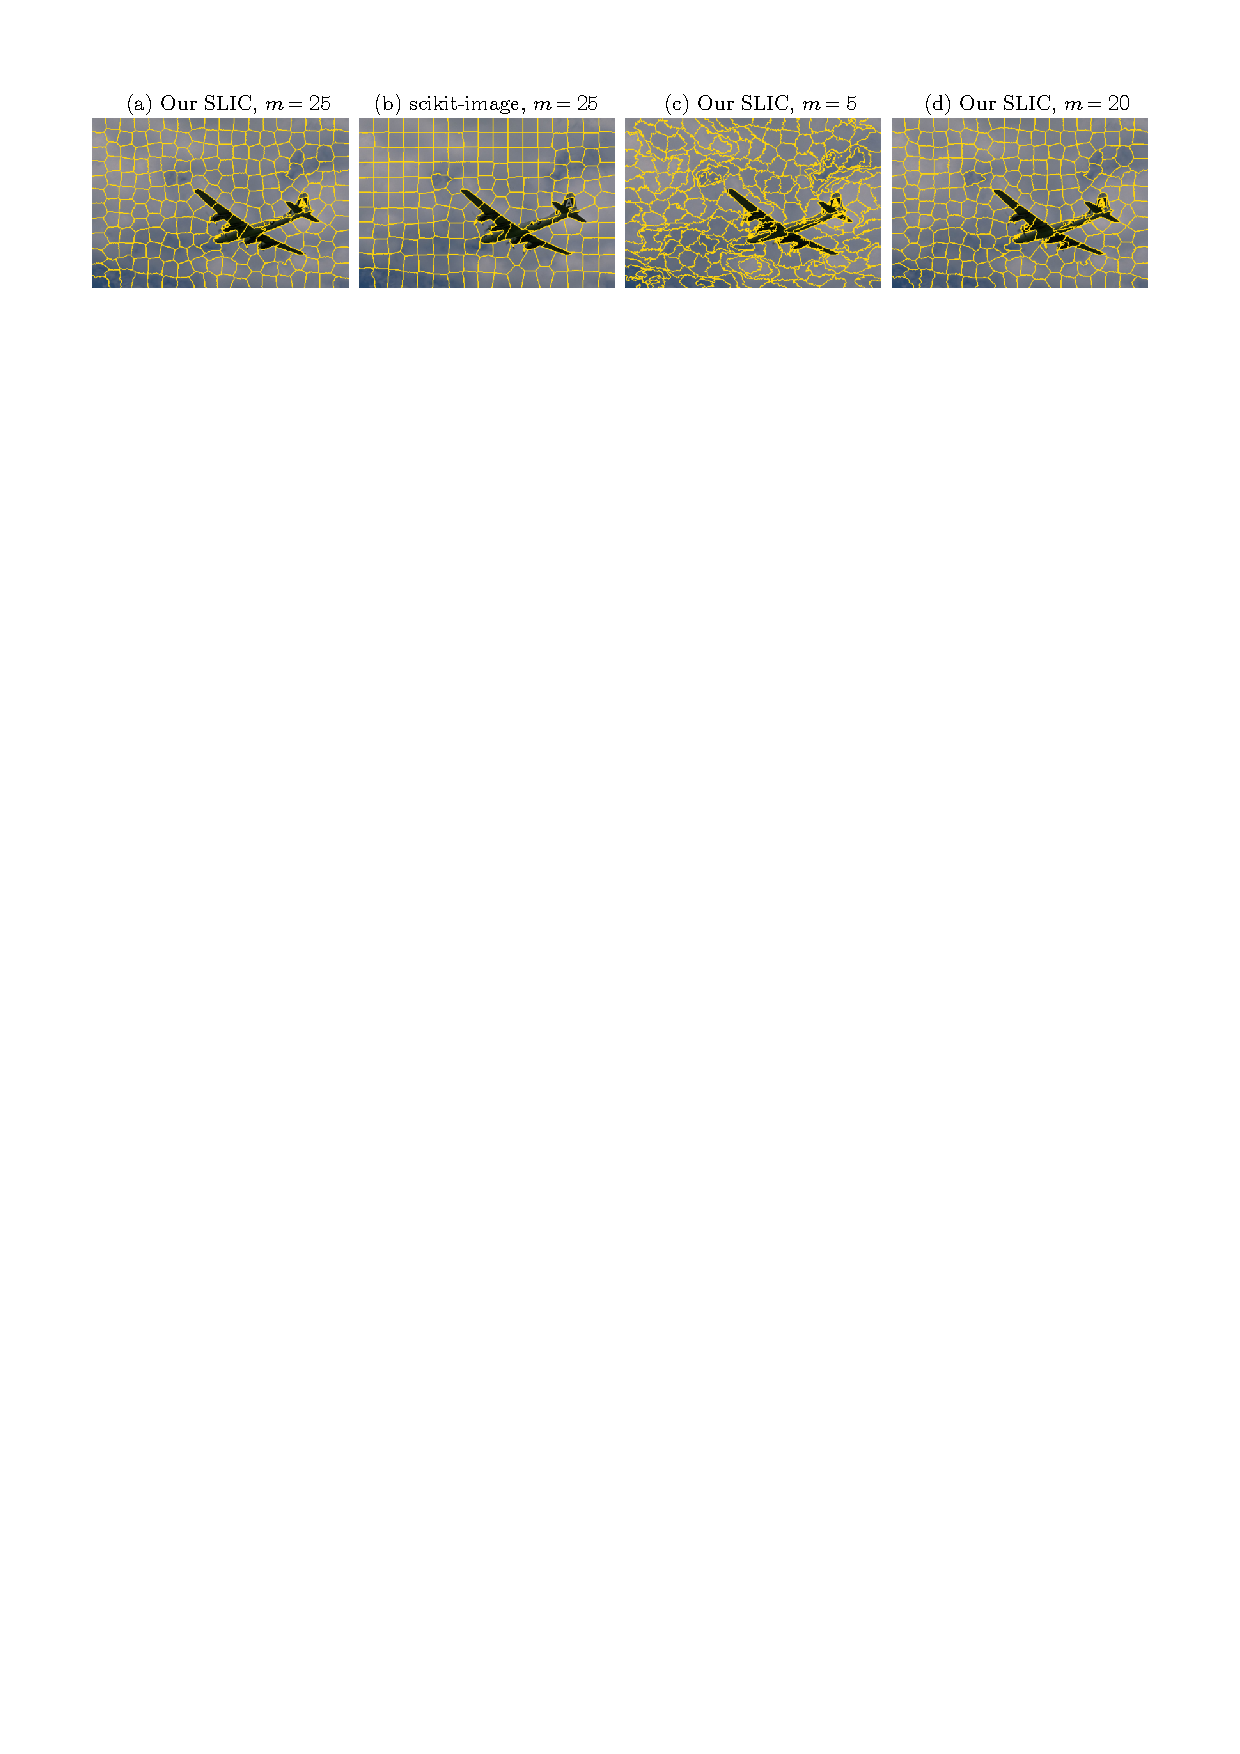
\includegraphics[width=\linewidth]{figs/slic-1}
\caption{Superpixels on image BSDS 3096 with $K = 200$. (a) and (b): our implementation and scikit-image for $m = 25$. (c)
and (d): our implementation for $m = 5$ and $m = 20$. With $m = 5$, color dominates and the boundaries follow the clouds, at the cost
of very irregular regions.}\label{f:visu}
\end{figure*}

\begin{figure*}[t]
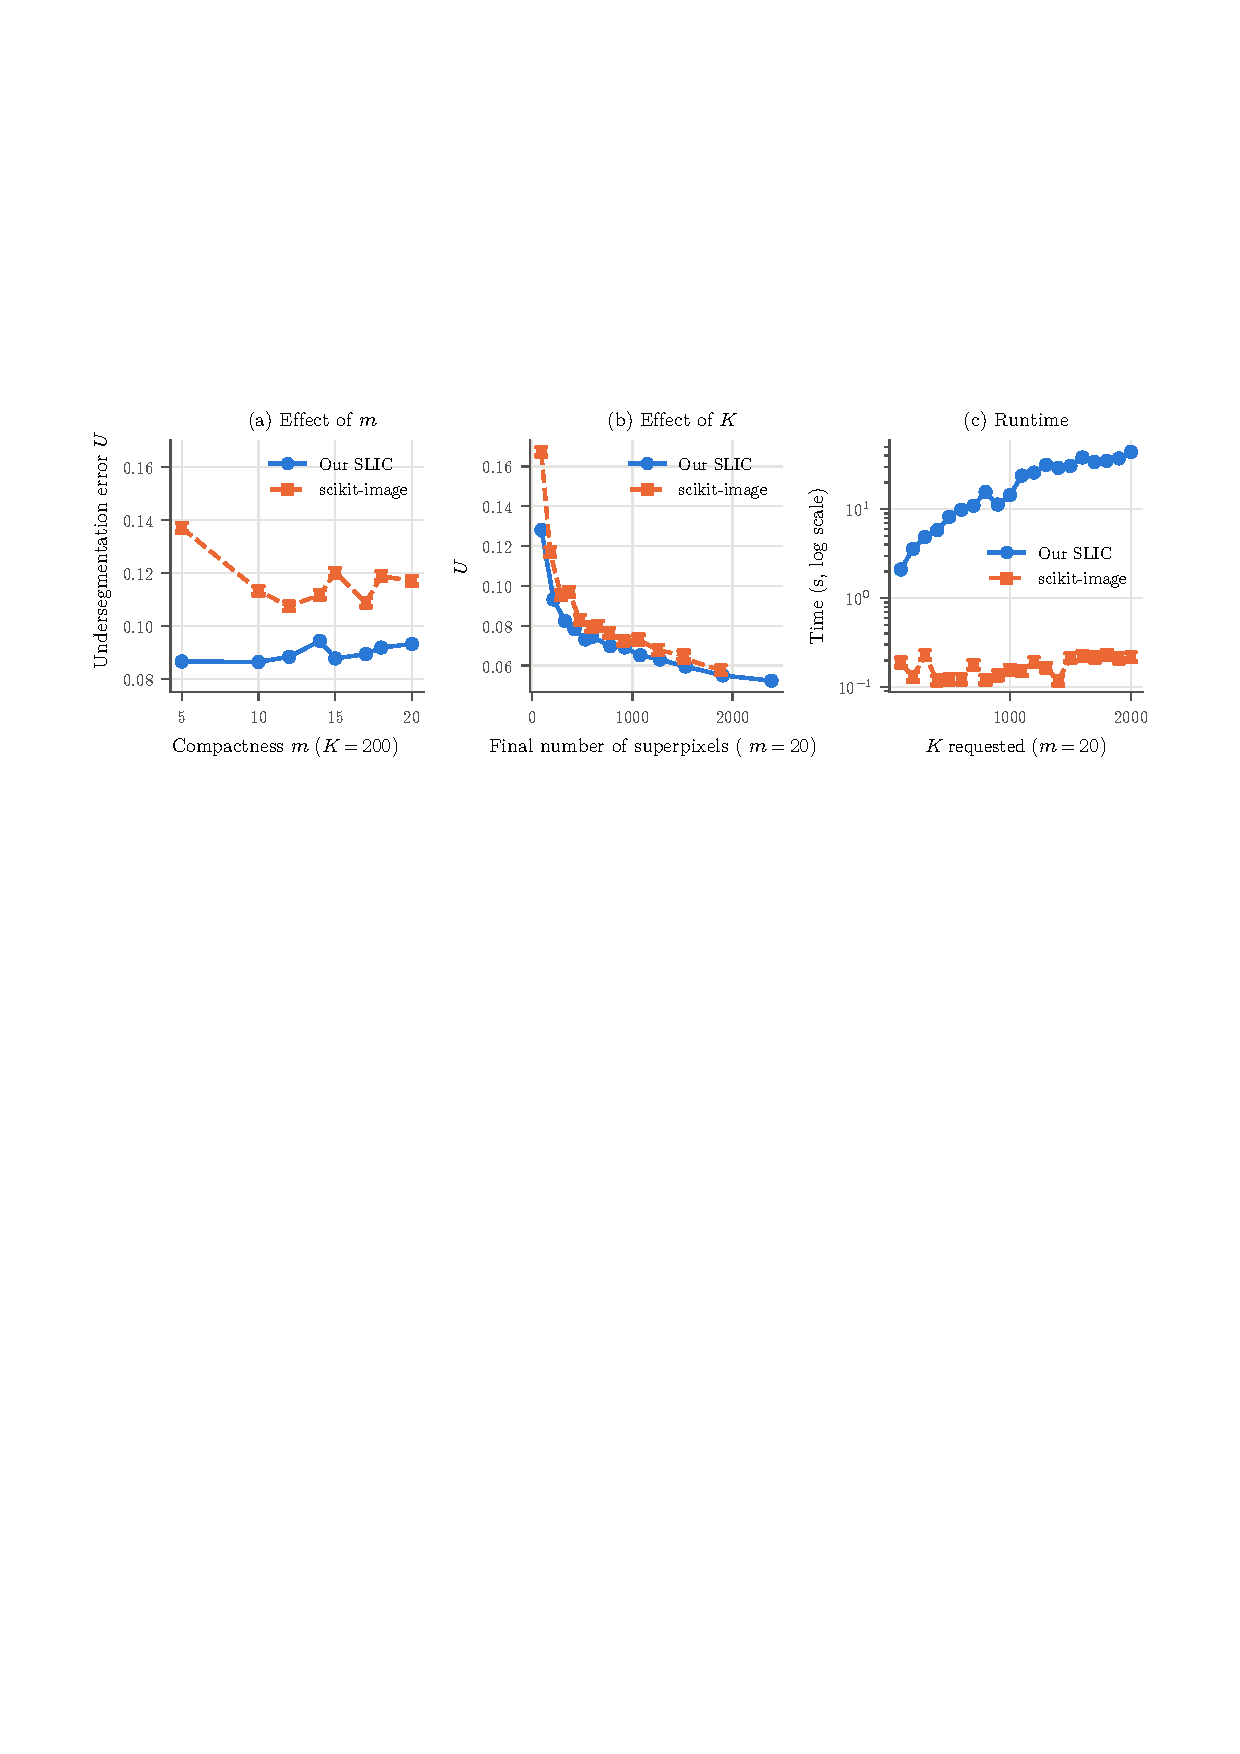
\includegraphics[width=\linewidth]{figs/slic-2}
\caption{Image BSDS 3096, error averaged over the five annotators. (a) Undersegmentation error versus the compactness $m$
for $K = 200$. (b) Error versus the final number of superpixels for $m = 20$. (c) Runtime versus $K$, on a logarithmic scale.}\label{f:courbes}
\end{figure*}

\section{Results on a Color Image}\label{s:color}
\subsection{Qualitative Comparison}
Figure~\ref{f:visu} shows the superpixels obtained for $K = 200$. For $m = 25$, our implementation and that of scikit-image
produce compact regions of similar size,
and both outline the silhouette of the plane, wings and
fuselage included. Our version produces 216 superpixels
versus 184 for scikit-image. The latter removes by default
the regions smaller than half the expected size,
whereas our threshold is one quarter.

The parameter $m$ clearly changes the look of the partition. With $m = 5$, the boundaries follow the gray
variations of the clouds and the regions take very
irregular shapes: the coefficient of variation of their size goes
from 0.18 for $m = 20$ to 0.33 for $m = 5$.

\subsection{Influence of Compactness}
On this image, the undersegmentation error stays
between 0.086 and 0.094 when $m$ goes from 5 to 20
(Figure~\ref{f:courbes}a). Compactness changes the look of the regions far
more than it changes their leakage: most
annotators split the sky into very few
regions, so following the outline of the clouds brings
almost nothing in terms of $U$. At $K = 200$ and $m = 25$, our
implementation obtains $U = 0.094$ versus 0.115 for
scikit-image. The gap holds for each of the five
annotators taken separately, from 0.028 to 0.226 for our version.

\subsection{Influence of the Number of Superpixels}
The error decreases steadily with the number of superpixels (Figure~\ref{f:courbes}b), from 0.128 for $K_f = 96$ to 0.052
for $K_f = 2386$. Smaller superpixels leak
less, which is the expected behavior. Both
implementations follow the same trend, and our version
keeps a lower error at a comparable number of superpixels. The plateaus of $K_f$ described in Section~\ref{s:impl} are
visible: $K = 1100$ and $K = 1200$ both give $K_f = 1274$.

\subsection{Runtime}
This is the weak point of our version (Figure~\ref{f:courbes}c): 2.1~s
for $K = 100$ and 44.2~s for $K = 2000$, versus 0.12 to
0.23~s for scikit-image. Part of the gap comes from Python
itself, since the connectivity check visits
the pixels one by one. The other part comes from the update
of the centers: for each center, we build a
mask over the whole image, which costs $O(NK)$ per iteration
instead of $O(N)$. This is the term that makes the
runtime grow with $K$. Accumulating the sums in a single
pass over the image, with \texttt{np.bincount}, would make this
step independent of $K$.

\section{Hyperspectral Extension}\label{s:hyper}
\subsection{Adapting the Method}
A hyperspectral image is an $h \times w \times B$ cube in which
each pixel carries a spectrum of $B$ bands. The Lab space
no longer makes sense, and we work directly on the spectra:
\begin{itemize}
\item the color distance becomes the Euclidean norm between spectra, $d_c = \lVert \mathbf{x}_i - \mathbf{x}_k \rVert_2$ over the $B$ bands;
\item the gradient of Equation~\eqref{e:G} sums the Sobel derivatives of the $B$ bands; for the gradient alignment,
it is computed on the cube normalized between 0 and 1;
\item the centers store a mean spectrum and a position, i.e.\ $B + 2$ components;
\item the initialization, the local assignment, the stopping criterion and
the connectivity check are unchanged.
\end{itemize}
The assignment remains $O(N)$ per iteration, but each comparison now costs $O(B)$.

\subsection{Data}
Salinas is an agricultural scene in California acquired
by the airborne AVIRIS sensor~\cite{ehu}. It measures $512 \times 217$ pixels and has 204 bands once the
water absorption bands are removed. Its ground truth distinguishes
16 crop classes, and the unlabeled pixels form
a background region. Pavia University is an urban scene
acquired by the ROSIS sensor~\cite{ehu}, of $610 \times 340$ pixels and
103 bands, with 9 labeled classes.

\begin{table}[t]
\caption{Salinas, metrics versus $m$ for $K = 200$ and versus
$K$ for $m = 20$. $U$ is computed with $B = 5\,\%$, BR denotes the boundary recall.}\label{t:salinas}
\centering\small
\begin{tabular}{rrrccc}
\toprule
$K$ & $m$ & $K_f$ & $U$ & BR & $GA$\\
\midrule
200 & 5 & 198 & 0.523 & 0.912 & 2.01\\
200 & 10 & 198 & 0.480 & 0.915 & 2.00\\
200 & 20 & 198 & 0.513 & 0.909 & 2.02\\
200 & 30 & 198 & 0.505 & 0.908 & 2.02\\
200 & 40 & 198 & 0.513 & 0.912 & 2.02\\
200 & 50 & 198 & 0.486 & 0.911 & 2.01\\
\midrule
50 & 20 & 55 & 0.814 & 0.780 & 2.65\\
100 & 20 & 112 & 0.602 & 0.866 & 2.10\\
200 & 20 & 198 & 0.513 & 0.909 & 2.02\\
500 & 20 & 549 & 0.362 & 0.964 & 1.62\\
1000 & 20 & 1107 & 0.322 & 0.979 & 1.45\\
2000 & 20 & 2228 & 0.247 & 0.994 & 1.29\\
\bottomrule
\end{tabular}
\end{table}

\subsection{Results on Salinas}
Figure~\ref{f:salinas} shows the partition for $K = 300$ and
$m = 10$. The large homogeneous plots are split
into regions that follow the field limits, with a
boundary recall of 0.927 and a gradient alignment
of 1.87. However, the boundaries are very jagged:
inside a single plot, the superpixels form irregular patterns.

\begin{figure}[t]
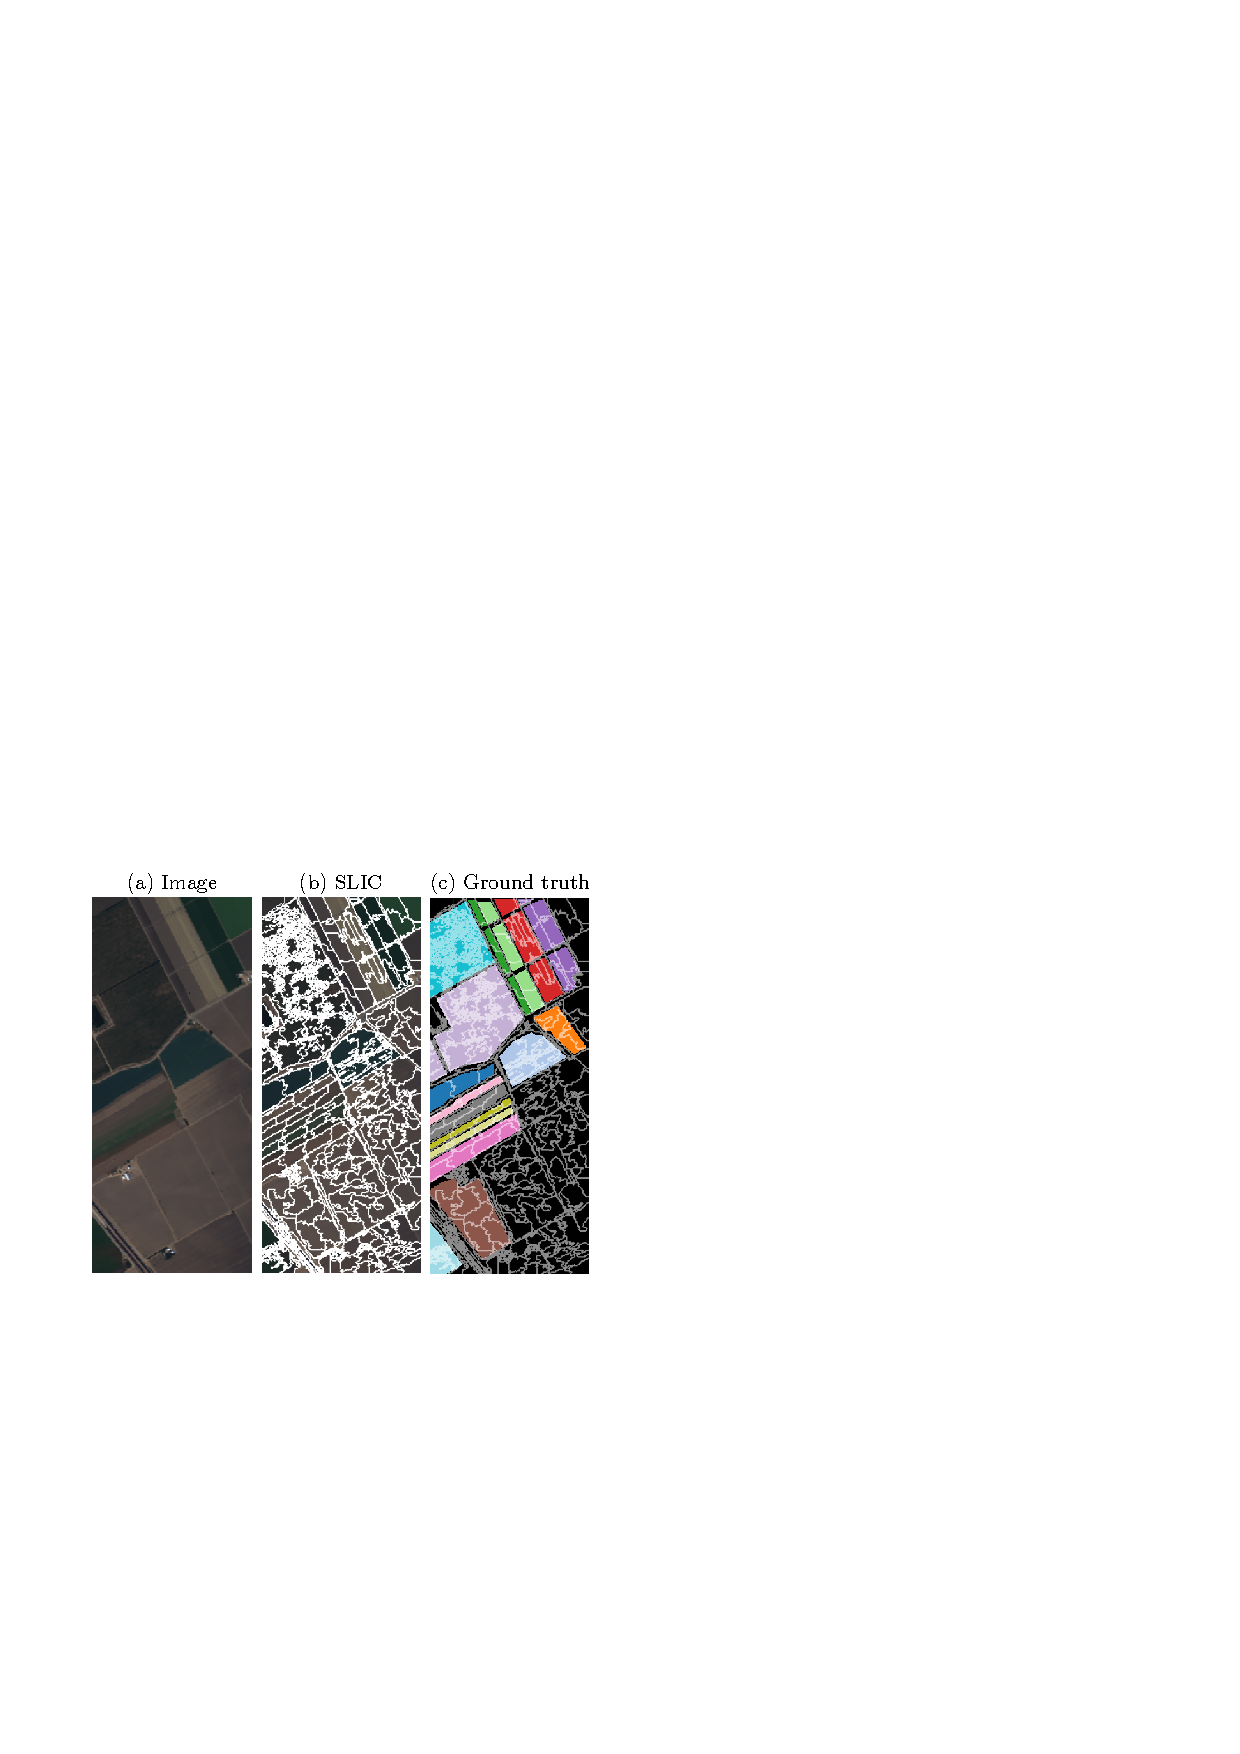
\includegraphics[width=\linewidth]{figs/slic-3}
\caption{Salinas. (a) Color composite of bands 29,
19 and 9. (b) Superpixels for $K = 300$ and $m = 10$. (c) Ground
truth, with the superpixel boundaries overlaid.}\label{f:salinas}
\end{figure}

Table~\ref{t:salinas} explains why. When $m$ goes from
5 to 50, the three metrics stay nearly constant: $U$
between 0.480 and 0.523, BR between 0.908 and 0.915. The spatial term
weighs almost nothing. The cube is indeed processed
in raw radiance, with values up to 9,207.
The median spectral distance between two pixels shifted
by half a grid step in each direction is 1,650,
whereas the spatial term $m\,d_s/S$ does not exceed $\sqrt{2}\,m$
in the search window, i.e.\ about 70 for $m = 50$.
Values of $m$ of the order of a thousand would be needed to
recover the balance intended by the paper. The range $[1, 40]$
only makes sense for the scale of CIELAB colors.

The number of superpixels, on the other hand, acts as
expected. From $K = 50$ to $K = 2000$, the error $U$ drops
from 0.814 to 0.247 and the recall rises from 0.780 to 0.994.
The gradient alignment decreases, from 2.65 to 1.29: with
smaller regions, a growing share of the boundaries
necessarily crosses homogeneous areas. The
runtime stays between 12 and 25~s over the whole range of $K$, without
growing with it: the assignment, which compares spectra
of 204 bands, costs the same whatever the value of $K$.

\subsection{Spectral Homogeneity on Pavia}
On Pavia, we studied what a superpixel contains rather than where its boundaries lie. The cube
is normalized between 0 and 1 and segmented with $K = 200$ and
$m = 1$ by a lighter variant of the implementation,
which runs ten iterations without a connectivity check.
It expresses the distance as $\sqrt{(d_c/m)^2 + (d_s/S)^2}$, which is
Equation~\eqref{e:D} divided by $m$ and therefore ranks the centers in
the same way. We obtain 209 superpixels, and the absence
of a connectivity check is clearly visible: a superpixel
is split into a median of 15 disjoint pieces, which
illustrates the role of the last step of the algorithm. For
each superpixel, we compute the standard deviation of each
band over its pixels, then the mean over the 103 bands, denoted $\bar\sigma$.

\begin{figure*}[t]
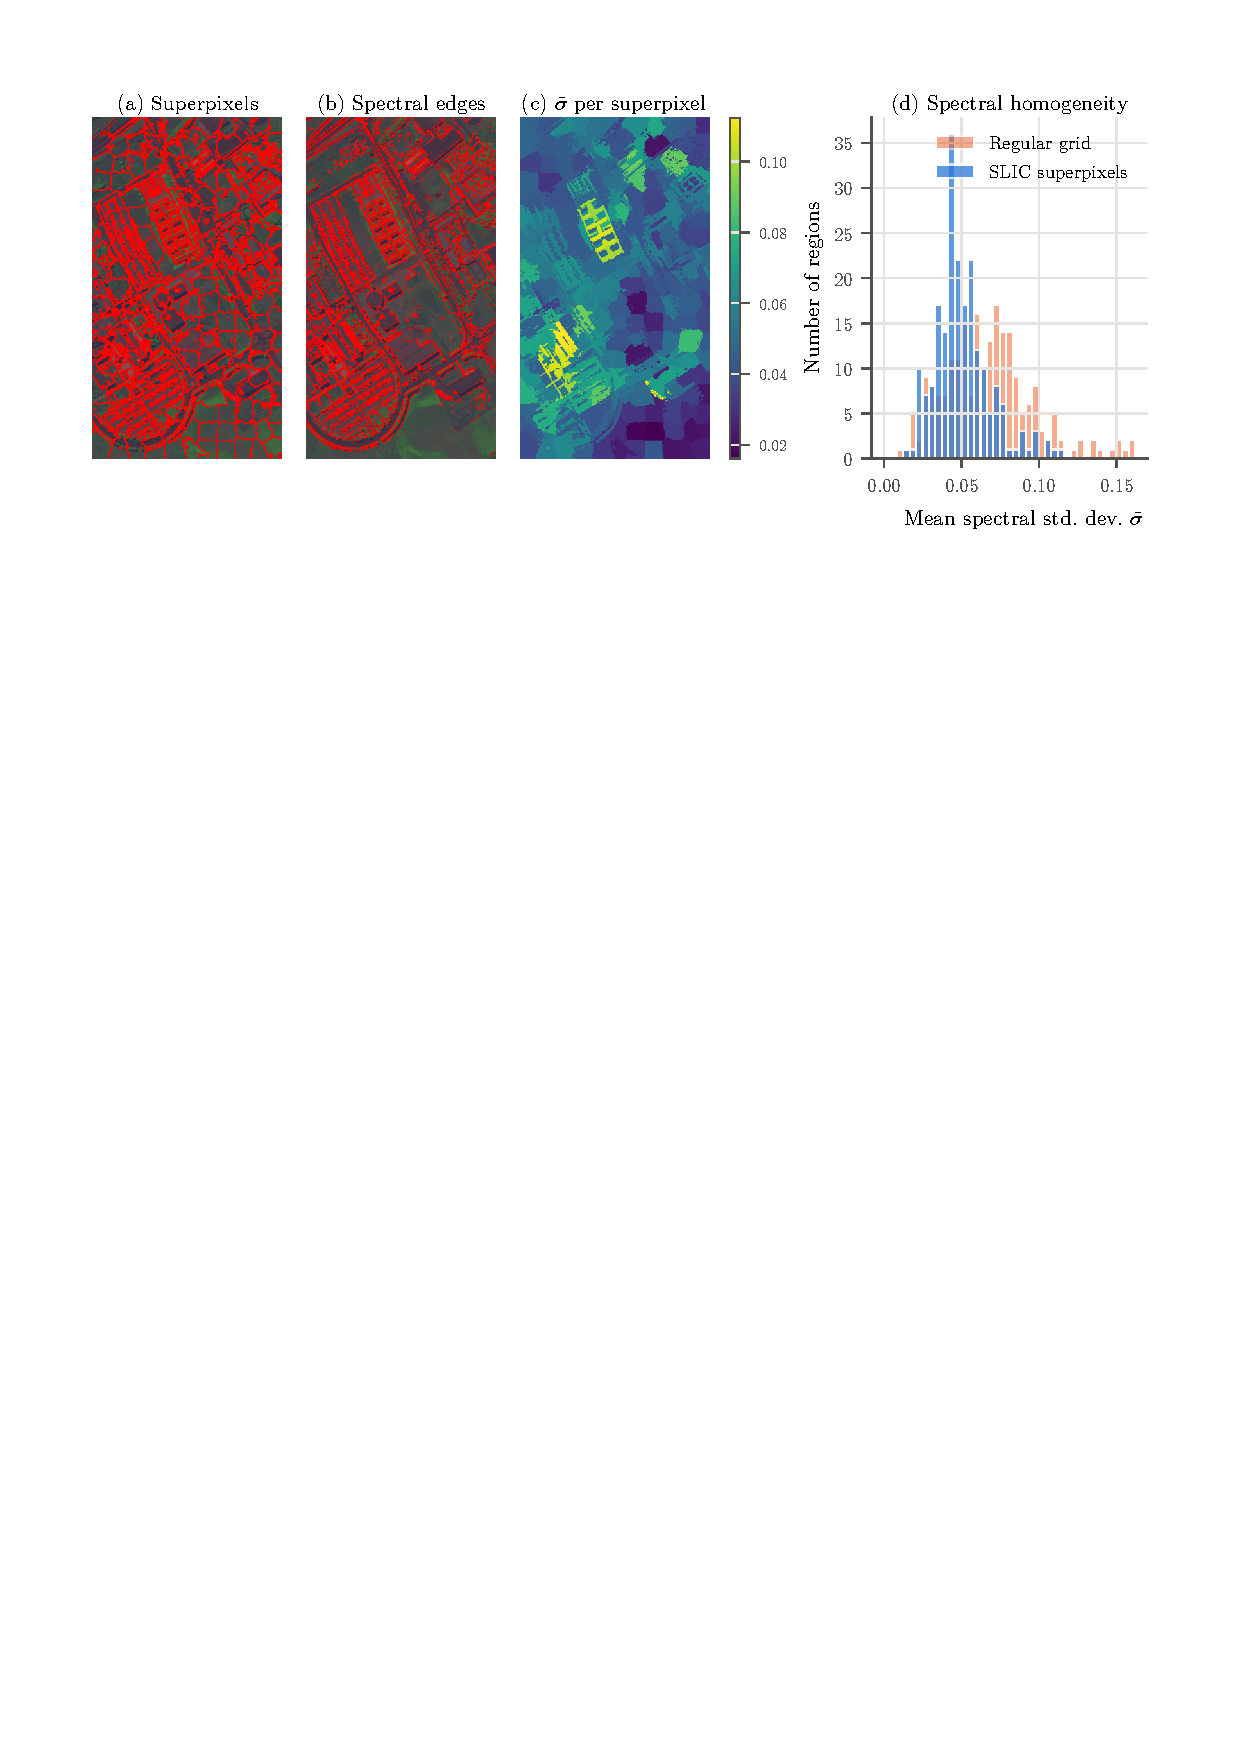
\includegraphics[width=\linewidth]{figs/slic-4}
\caption{Pavia University, $K = 200$ and $m = 1$ on the normalized cube. (a) Superpixel boundaries on a color
composite of the first three principal components. (b) Spectral edges, obtained by thresholding the spectral gradient. (c) Mean
spectral standard deviation of each superpixel. (d) Distribution of this standard deviation for the superpixels and for a regular grid of blocks
of the same size.}\label{f:pavia}
\end{figure*}

Figure~\ref{f:pavia} shows that the superpixels follow the buildings, the roads and the vegetation areas picked out by
the spectral edges. Their median spectral standard deviation
is 0.0468, versus 0.0663 for a regular grid of
blocks of the same mean size. Against the 9 classes of
the ground truth, the mean purity of the superpixels, i.e.\ the share of their labeled pixels that belongs to the
majority class, reaches 93\,\% versus 85\,\% for the grid.
The comparison slightly favors SLIC, since its fragmented superpixels can gather similar pixels
that do not touch. The first three principal components
carry 98.9\,\% of the variance of the cube, which
confirms that the spectral information is highly redundant and that a dimensionality reduction before SLIC would be possible.

\section{Extension to Volumes}\label{s:vol}
\subsection{Supervoxels}
The paper mentions the extension of SLIC to videos and
volumes. The changes are straightforward:
\begin{itemize}
\item the grid step becomes $S = \sqrt[3]{N/K}$ and the centers form a cubic grid;
\item the initial move looks for the gradient minimum in a $3 \times 3 \times 3$ neighborhood;
\item the search window becomes a $2S \times 2S \times 2S$ cube and $d_s$ a three-dimensional distance;
\item the connectivity check uses the 6-voxel neighborhood and a threshold of $S^3/4$ voxels.
\end{itemize}
The metrics extend in the same way: the boundaries
become surfaces and the recall is computed with a tolerance of one voxel.

\begin{table}[t]
\caption{Supervoxels, $K = 200$. For the sphere, the ground
truth is the ball and the background. For the MRI, it separates gray
matter, white matter and the rest of the volume.}\label{t:vox}
\centering\small
\begin{tabular}{lrccc}
\toprule
Volume & $m$ & $U$ & BR & $GA$\\
\midrule
Sphere & 0.50 & 0.000 & 1.000 & 1.22\\
Sphere & 1 & 0.105 & 0.932 & 1.11\\
Sphere & 2 & 0.143 & 0.715 & 1.01\\
Sphere & 5 & 0.150 & 0.667 & 0.99\\
Sphere & 10 & 0.150 & 0.662 & 0.99\\
Sphere & 20 & 0.150 & 0.661 & 0.99\\
\midrule
MRI & 0.25 & 0.350 & 0.781 & 1.93\\
MRI & 0.50 & 0.388 & 0.629 & 1.76\\
MRI & 1 & 0.419 & 0.564 & 1.56\\
MRI & 2 & 0.421 & 0.562 & 1.17\\
MRI & 10 & 0.442 & 0.565 & 1.04\\
\bottomrule
\end{tabular}
\end{table}

\subsection{Data and Results}
We test the supervoxels on two volumes normalized between 0 and 1. The first is synthetic: a
ball of intensity 0.8 in a background at 0.2, on a grid
of $30 \times 100 \times 100$ voxels, with Gaussian noise of standard deviation 0.05,
the whole renormalized between 0 and 1. The second is
a slab of 10 axial slices of the MNI152 T1 brain template~\cite{fonov},
of $10 \times 233 \times 197$ voxels, whose gray and white matter
probability maps, thresholded at 0.5, serve as the reference.

\begin{figure}[t]
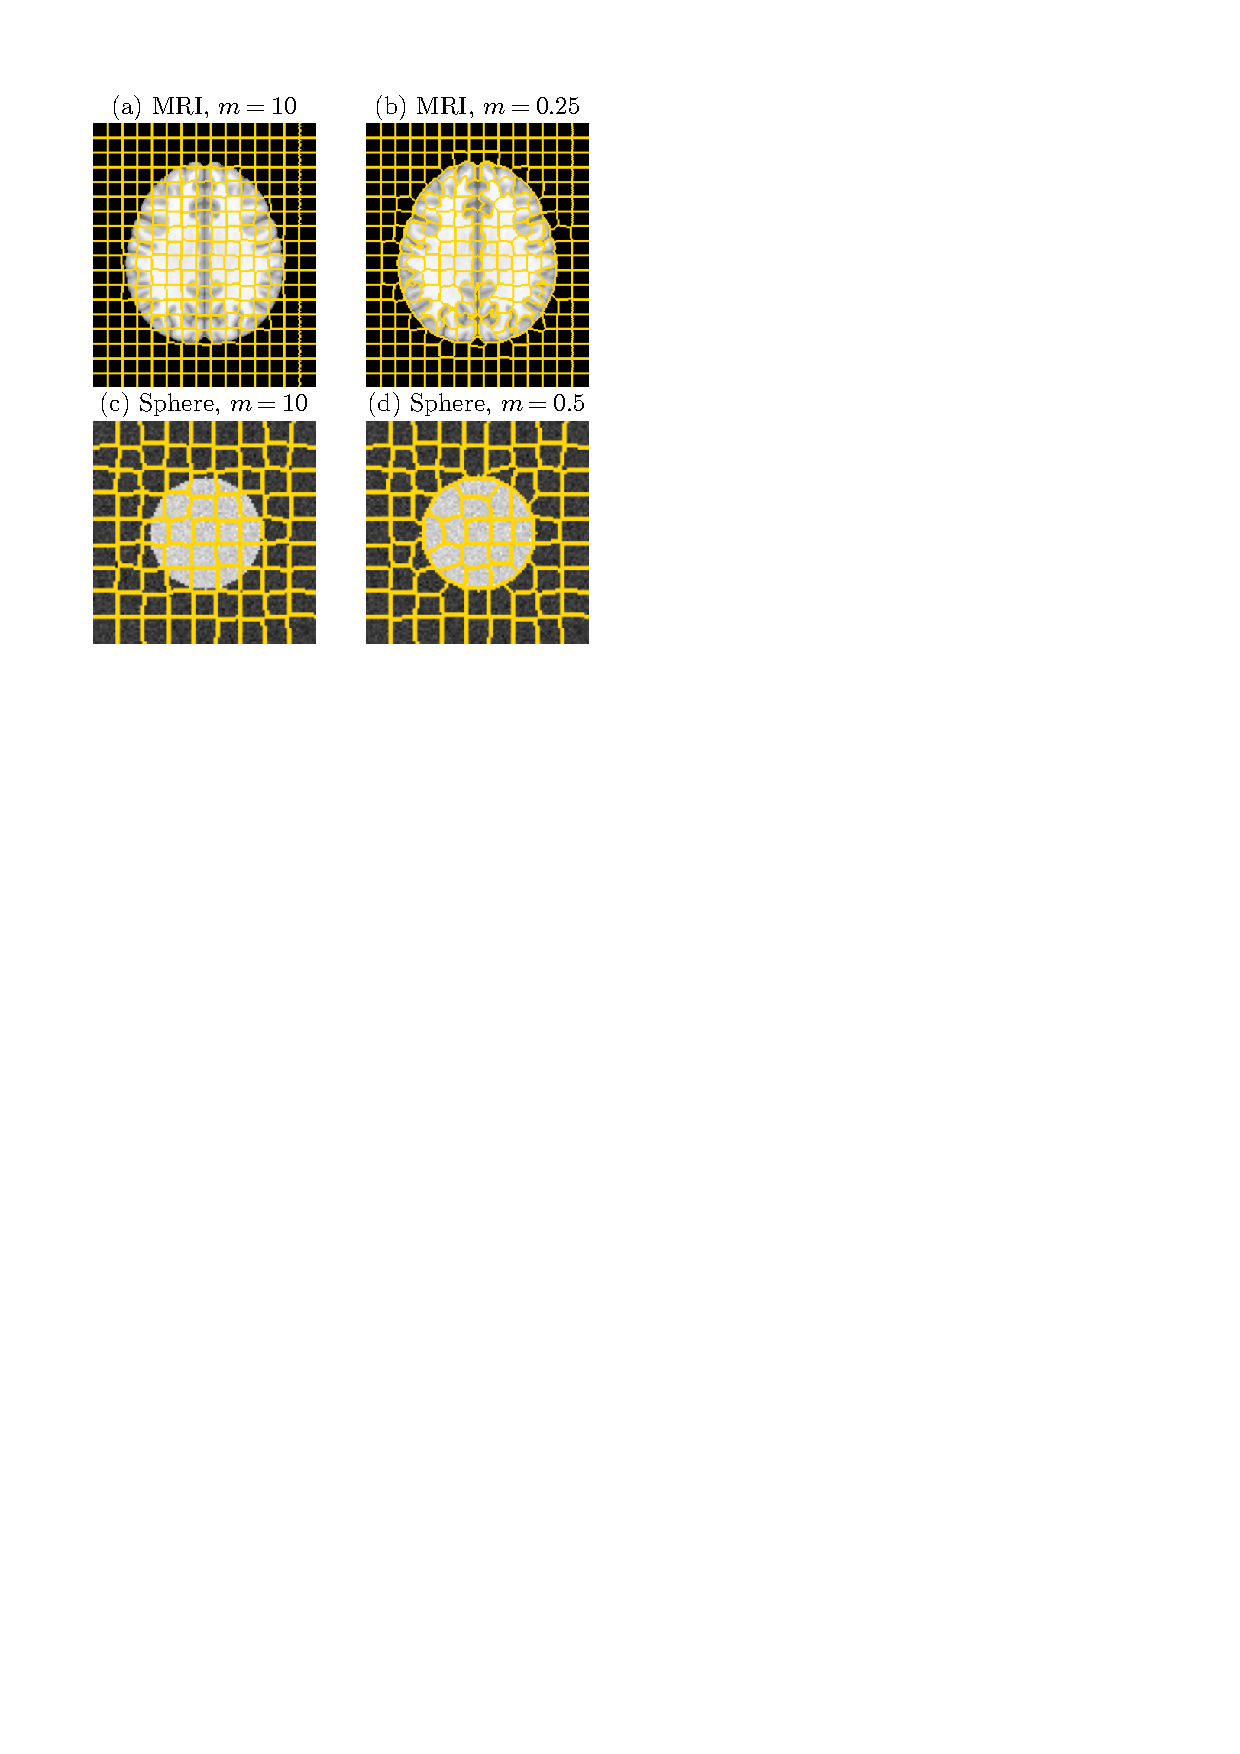
\includegraphics[width=\linewidth]{figs/slic-5}
\caption{Central slices of the supervoxels for $K = 200$.
(a) and (b): T1-weighted MRI slab. (c) and (d): noisy synthetic
sphere. With $m = 10$, the supervoxels remain
cubes; with an $m$ suited to the $[0, 1]$ scale, they follow the boundaries.}\label{f:vox}
\end{figure}

The same phenomenon as on Salinas appears, in
the opposite direction. The intensity gap between two tissues does not exceed
1, whereas the spatial term $m\,d_s/S$ reaches
$\sqrt{3}\,m$ in the search window. With $m = 10$, position
dominates and the supervoxels remain cubes aligned
with the grid (Figure~\ref{f:vox}a and~c). On the sphere, the boundary
recall is only 0.662. Lowering $m$ to 0.5, the
supervoxels follow the ball exactly: $U$ drops to
0.000 and the recall reaches 1.000 (Table~\ref{t:vox}). On the MRI,
going from $m = 10$ to $m = 0.25$ raises the boundary recall
from 0.565 to 0.781 and the gradient alignment from
1.04 to 1.93. The supervoxels then follow the outline of the
brain and its internal structures (Figure~\ref{f:vox}b).

At a fixed $m = 10$ on the sphere, increasing $K$ from 50 to
800 takes $U$ from 0.256 to 0.107 and the recall from 0.514
to 0.931: more supervoxels partly make up for a
poorly tuned compactness, but at a much higher cost in memory and time.

\section{Discussion and Limitations}\label{s:disc}
\pa{Tuning $m$.} This is the main lesson of the
project. Equation~\eqref{e:D} compares a distance in the space
of values to a normalized spatial distance, and $m$ only makes
sense relative to the scale of those values. The range
of the paper holds for CIELAB colors. It is already
shifted by OpenCV's 8-bit Lab conversion, which
stretches the lightness from $[0, 100]$ to $[0, 255]$, which partly explains
the weak effect of $m$ on the BSDS image. It
becomes too small by one or two orders of magnitude
for a raw hyperspectral radiance, and too large
for normalized volumes. A simple rule is
to normalize the data, then to choose $m$ from the
typical spectral distance between neighboring pixels, measured
on the image itself. The SLICO variant of the paper,
which adapts $m$ to each superpixel, goes in this direction.

\pa{The spectral distance.} The Euclidean norm on
radiances confuses a difference in material with
a mere difference in illumination, which multiplies the whole
spectrum by the same factor. The angular distance
of the Spectral Angle Mapper~\cite{kruse} is insensitive to it and would be
more relevant for shadowed scenes such as Pavia.
Reducing the cube to its first principal components
before SLIC would also divide the cost of each comparison.

\pa{The computational cost.} Our implementation remains slow,
because of the Python loops of the connectivity check and
of the $O(NK)$ update of the centers. These two steps
can be vectorized, or compiled with Numba, without changing the algorithm.

\pa{The evaluation.} The color results cover a
single image, and the metric $U$ depends on the partition
chosen by the annotators. On image 3096, the sky is
split into very few regions by most
annotators, which makes $U$ barely sensitive to $m$. An evaluation
on the whole Berkeley dataset, as in
the paper, would give more representative curves. In
three dimensions, the MRI reference is itself approximate since it comes from thresholded probability maps.

\section{Conclusion}
This project reimplemented SLIC in full, from the initialization on the gradient minimum to the
connectivity check. On image BSDS 3096, our version obtains
a slightly lower undersegmentation error
than scikit-image with equal parameters, with
regions of comparable visual quality, but a much longer runtime.

The extensions show that the method generalizes
easily. Moving to spectra and to volumes
changes neither the structure of the algorithm nor its linear
complexity. They also show that its simplicity has a price:
the whole balance between boundary adherence and regularity
rests on a parameter $m$ whose relevant value
depends on the scale of the data. Well tuned, SLIC cleanly splits
a hyperspectral scene of 204 bands or
a three-dimensional MRI. Poorly tuned, it ignores
position, as on Salinas in raw radiance, or ignores
the signal, as on the normalized volumes with $m = 10$.

{\small
\begin{thebibliography}{9}\setlength{\itemsep}{1pt}
\bibitem{achanta} R. Achanta, A. Shaji, K. Smith, A. Lucchi, P. Fua and S. Süsstrunk, ``SLIC Superpixels Compared to State-of-the-Art Superpixel Methods,'' \emph{IEEE Transactions on Pattern Analysis and Machine Intelligence}, vol.~34, no.~11, pp.~2274--2282, 2012.
\bibitem{martin} D. Martin, C. Fowlkes, D. Tal and J. Malik, ``A Database of Human Segmented Natural Images and its Application to Evaluating Segmentation Algorithms and Measuring Ecological Statistics,'' \emph{ICCV}, IEEE, 2001.
\bibitem{arbelaez} P. Arbeláez, M. Maire, C. Fowlkes and J. Malik, ``Contour Detection and Hierarchical Image Segmentation,'' \emph{IEEE Transactions on Pattern Analysis and Machine Intelligence}, vol.~33, no.~5, pp.~898--916, 2011.
\bibitem{felzenszwalb} P. Felzenszwalb and D. Huttenlocher, ``Efficient Graph-Based Image Segmentation,'' \emph{International Journal of Computer Vision}, vol.~59, no.~2, pp.~167--181, 2004.
\bibitem{skimage} S. van der Walt et al., ``scikit-image: Image Processing in Python,'' \emph{PeerJ}, vol.~2, e453, 2014.
\bibitem{ehu} Grupo de Inteligencia Computacional, Universidad del País Vasco, ``Hyperspectral Remote Sensing Scenes,'' Salinas and Pavia University datasets.
\bibitem{fonov} V. Fonov, A. C. Evans, K. Botteron, C. R. Almli, R. C. McKinstry and D. L. Collins, ``Unbiased Average Age-Appropriate Atlases for Pediatric Studies,'' \emph{NeuroImage}, vol.~54, no.~1, pp.~313--327, 2011.
\bibitem{kruse} F. A. Kruse et al., ``The Spectral Image Processing System (SIPS): Interactive Visualization and Analysis of Imaging Spectrometer Data,'' \emph{Remote Sensing of Environment}, vol.~44, no.~2--3, pp.~145--163, 1993.
\end{thebibliography}}
\end{document}
